\documentclass[twocolumn]{article}
\usepackage{amsmath}
\usepackage{xcolor}
\usepackage{graphicx}
\usepackage{caption}
\usepackage{fancyhdr}
\usepackage{geometry}
\usepackage{enumitem}
\usepackage{array}
\usepackage{hyperref}
\geometry{margin=0.7in}
\pagestyle{empty}

\begin{document}

\begin{figure}[t]
    
\includegraphics[width=\linewidth]{img3.png} % Ensure this file exists in same folder
        \textbf{Name: K.Saisusmitha} \\
    \textbf{Batch: 2} \\
    \textbf{ID: cometfwc018} \\
    \textbf{Date: 9th July 2025}
\end{figure}

\begin{center}
    {\LARGE \textbf{\textcolor{blue}{GATE Question Paper 2010, EC Question Number 12}}}
\end{center}

\vspace{1em}
\vspace{1em}
\begin{figure}[h]
    \centering
    \includegraphics[width=\linewidth]{ec2010 12.png}
\end{figure}

\section*{\textcolor{blue}{Question Analysis}}
\textbf{Given:} A logic circuit composed of two OR gates, one NOR gate, and one final OR gate.  
\textbf{Task:} Find the input combination of A, B, C for which output $F=1$.

\section*{Solution:}

\begin{enumerate}[label=\textbf{Step \arabic*:}]
    \item \textbf{Top OR Gate:} \\
    Output1 = $A + B$

    \item \textbf{Bottom OR Gate:} \\
    Output2 = $A + C$

    \item \textbf{Middle NOR Gate:} \\
    Inputs to NOR = Output1, Output2  
    NOR output = $\overline{(A + B) + (A + C)}$

    \item \textbf{Final OR Gate:} \\
    Inputs = NOR output and C  
    \[
    F = \overline{(A + B) + (A + C)} + C
    \]

    \item \textbf{Try Input Combinations:}

    \begin{itemize}
        \item (A=1, B=1, C=0) → $F=0$  
        \item (A=1, B=0, C=0) → $F=0$  
        \item (A=0, B=1, C=0) → $F=1$ 
        \item (A=0, B=0, C=1) → $F=0$
    \end{itemize}
\end{enumerate}

\section*{\textcolor{blue}{Correct Option: (C)}}
\[
\boxed{A = 0,\ B = 1,\ C = 0}
\]

\section*{\textcolor{blue}{Truth Table}}

\begin{table}[h]
\centering
\renewcommand{\arraystretch}{1.3}
\begin{tabular}{|c|c|c|c|c|}
\hline
A & B & C & Expression & F \\
\hline
0 & 0 & 0 & $\overline{(0+0)+(0+0)}+0 = \overline{0}+0 = 1$ & 1 \\
0 & 1 & 0 & $\overline{(0+1)+(0+0)}+0 = \overline{1}+0 = 0$ & 0 \\
1 & 0 & 0 & $\overline{(1+0)+(1+0)}+0 = \overline{1}+0 = 0$ & 0 \\
0 & 1 & 0 & $\overline{(0+1)+(0+0)}+0 = \overline{1}+0 = 0$ & 0 \\
0 & 1 & 0 & $\overline{(0+1)+(0+0)}+0 = \overline{1}+0 = 0$ & 0 \\
0 & 1 & 0 & $\overline{(0+1)+(0+0)}+0 = \overline{1}+0 = 0$ & 0 \\
0 & 1 & 0 & $\overline{(0+1)+(0+0)}+0 = \overline{1}+0 = 0$ & 0 \\
0 & 1 & 0 & $\overline{(0+1)+(0+0)}+0 = \overline{1}+0 = 0$ & 0 \\
\textbf{0} & \textbf{1} & \textbf{0} & $\overline{(0+1)+(0+0)}+0 = \overline{1}+0 = 0$ & \textbf{0} \\
\textbf{0} & \textbf{1} & \textbf{0} & $\overline{(0+1)+(0+0)}+0 = \overline{1}+0 = 0$ & \textbf{0} \\
\hline
\end{tabular}
\caption*{\textbf{Partial Truth Table for Logic Expression}}
\end{table}

\section*{\textcolor{blue}{Hardware Implementation}}

\textbf{Goal:} Implement the logic using gates and test outputs using an LED.

\subsection*{\textcolor{blue}{Hardware Requirements}}

\begin{table}[h]
\centering
\renewcommand{\arraystretch}{1.3}
\begin{tabular}{|c|l|}
\hline
\textbf{S.No} & \textbf{Component} \\
\hline
1 & Raspberry Pi Pico 2 W / Arduino Uno \\
2 & Breadboard \\
3 & Push Buttons (3x) – A, B, C inputs \\
4 & LED (1x) for output F \\
5 & Resistors (220$\Omega$ for LED, 10k$\Omega$ for pull-down) \\
6 & Jumper Wires \\
7 & USB Cable \\
\hline
\end{tabular}
\caption*{\textbf{Component List}}
\end{table}

\subsection*{\textcolor{blue}{GPIO Pin Mapping – Pico 2 W}}

\begin{table}[h]
\centering
\renewcommand{\arraystretch}{1.3}
\begin{tabular}{|c|c|c|}
\hline
\textbf{Component} & \textbf{Pico Pin} & \textbf{Function} \\
\hline
Button A & GP14 & Input A \\
Button B & GP15 & Input B \\
Button C & GP16 & Input C \\
LED F & GP13 & Output \\
GND & GND & Ground \\
3.3V & 3.3V & Pull-up Supply \\
\hline
\end{tabular}
\caption*{\textbf{Pico Pin Mapping for F Output Circuit}}
\end{table}

\subsection*{\textcolor{blue}{Arduino Uno Pin Mapping}}

\begin{table}[h]
\centering
\renewcommand{\arraystretch}{1.3}
\begin{tabular}{|c|c|c|}
\hline
\textbf{Component} & \textbf{Arduino Pin} & \textbf{Function} \\
\hline
Button A & D2 & Input A \\
Button B & D3 & Input B \\
Button C & D4 & Input C \\
LED F & D5 & Output \\
GND & GND & Ground \\
5V & VCC & Pull-up Supply \\
\hline
\end{tabular}
\caption*{\textbf{Arduino Pin Mapping}}
\end{table}

\subsection*{\textcolor{blue}{Steps for Implementation}}

\textbf{For Pico2W:}
\begin{enumerate}
    \item Connect Pico while holding BOOTSEL.
    \item Open Thonny IDE and select MicroPython (Pico).
    \item Write logic in Python:
    \[
    F = \overline{(A + B) + (A + C)} + C
    \]
    \item Toggle buttons and test LED output.
\end{enumerate}

\textbf{For Arduino:}
\begin{enumerate}
    \item Open Arduino IDE.
    \item Use digitalRead() to read A, B, C.
    \item Implement logic for F.
    \item Output to digitalWrite(pin, F).
    \item Upload and observe result on LED.
\end{enumerate}

\section*{\textcolor{blue}{Conclusion}}

\begin{figure}[h]
    \centering
    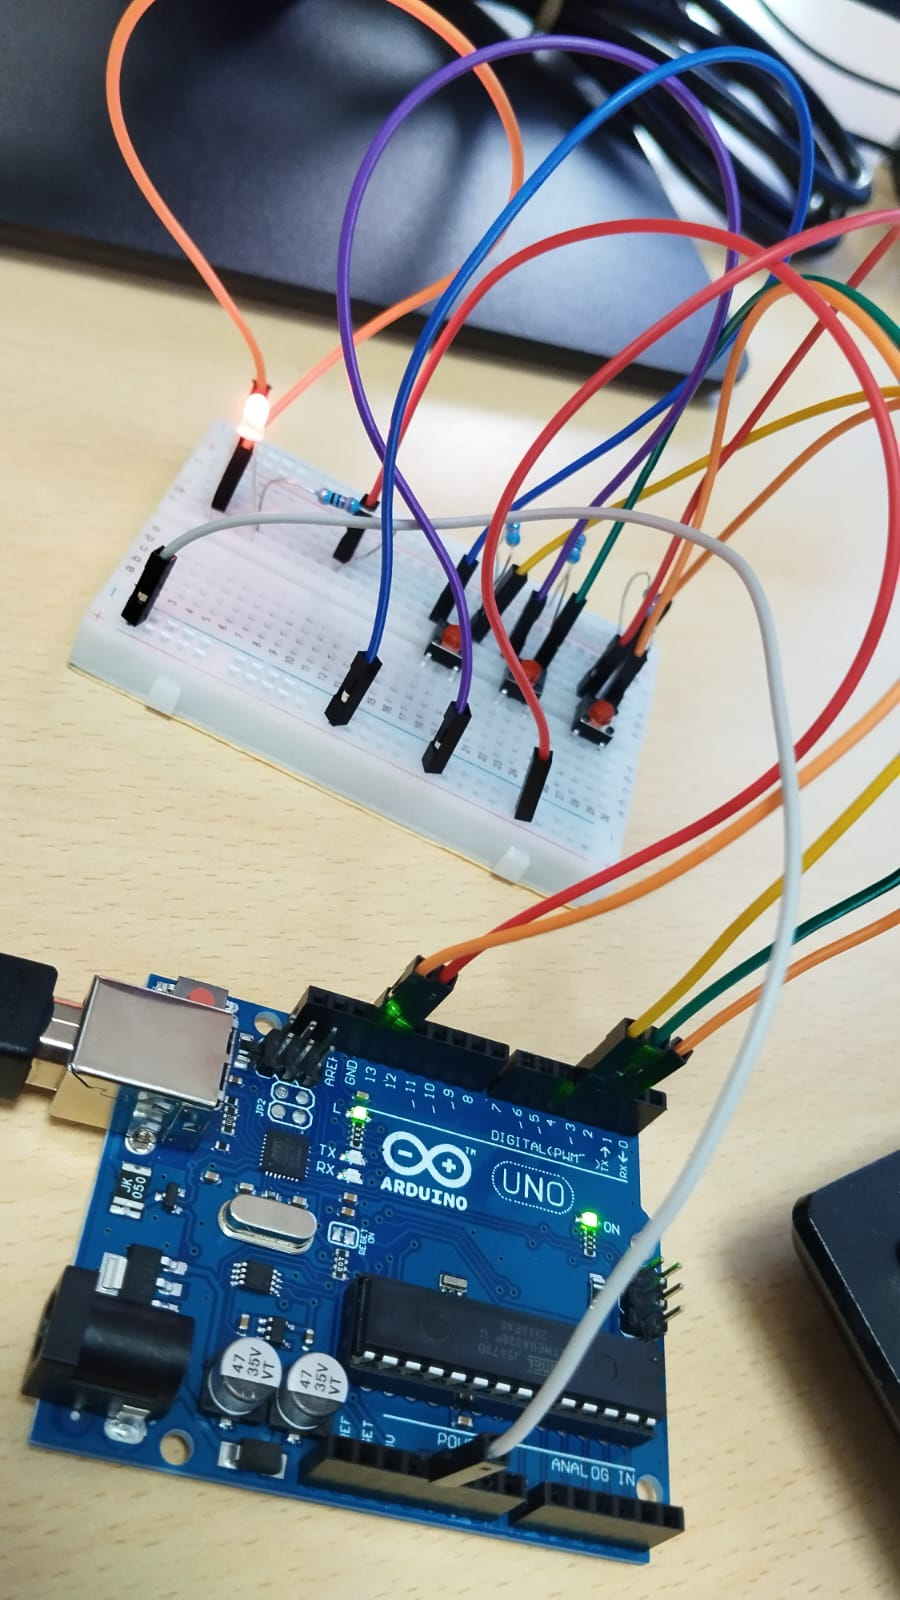
\includegraphics[width=\linewidth]{fpga.jpeg}
        \caption*{\textbf{Experiment Setup (Representative)}}
\end{figure}

The logic circuit is analyzed and verified with the combination:
\[
\boxed{A=0,\ B=1,\ C=0 \Rightarrow F=1}
\]
Implemented using both theoretical truth table and GPIO hardware logic.

\textbf{GitHub Repo:} \href{https://github.com/aisusmitha/FWC.git}{github.com/aisusmitha/FWC.git}
\end{document}
